\documentclass[11pt]{article}
\usepackage[margin=1in]{geometry}
\usepackage[T1]{fontenc}
\usepackage{lmodern}
\usepackage{booktabs}
\usepackage{graphicx}
\usepackage{xcolor}
\usepackage{amsmath}
\usepackage[hidelinks]{hyperref}
\usepackage{url}

% Placeholders are red and loud on purpose: a paper with a visible TODO cannot be submitted by accident.
\newcommand{\todo}[1]{\textcolor{red}{\textbf{[TODO: #1]}}}
\InputIfFileExists{generated/numbers.tex}{}{\newcommand{\TwentySevenAgentCOneBase}{\todo{run make\_results.py}}}

\title{Serving Small Hybrid-Attention Language Models for Agent Workloads:\\
An Empirical Study of Inference-Engine Configuration\\
\large (working title; see \S\ref{sec:scope} for what this version does and does not claim)}
\author{\todo{author names and affiliations}}
\date{\todo{date}}

\begin{document}
\maketitle

\begin{abstract}
We measure how inference-engine configuration changes the throughput and tail latency of two small open-weight models,
Qwen3.8-27B-FP8 on one H100 and Qwen3.5-9B on one L40S, served with vLLM under traffic shaped like agent loops (a long shared
system prompt and multi-turn sessions with growing history). We define the vanilla baseline as engine defaults plus only the
flags needed to start, vary one setting at a time, and report throughput and p99 time to first token.
On the 27B model, speculative decoding with the model's built-in multi-token-prediction head and three draft tokens raised
single-stream agent-session throughput from \TwentySevenAgentCOneBase{} to \TwentySevenAgentCOneBest{} output tokens per second
(\TwentySevenAgentCOneGain\%) and concurrency-16 throughput from \TwentySevenAgentCSixteenBase{} to \TwentySevenAgentCSixteenBest{}
(\TwentySevenAgentCSixteenGain\%).
We also report that vanilla vLLM~0.33.0 cannot start the 27B model on an H100 because its default sequence limit exceeds the
number of recurrent-state cache blocks that fit in memory.
On a 200-question GSM8K sample, answer accuracy with speculation was unchanged within sampling noise (27B: 0.940 to 0.935; 9B: 0.900 to 0.910).
\end{abstract}

\section{Introduction}
Agent workloads stress an inference engine differently from the single-prompt benchmarks that engine defaults are usually
tuned on. Requests repeat a long system prompt, arrive as multi-turn sessions whose prefix grows, and mix short tool calls with
longer reasoning. Recent small models also use hybrid attention with linear-attention layers, which changes what limits
concurrency: Qwen3.8-27B uses linear attention on 48 of its 64 layers~\cite{qwen38_card}, so per-sequence recurrent state, not only
the key-value cache, bounds how many sequences an engine can hold.

This report is an empirical configuration study with a deliberately narrow scope. Its contributions are:
\begin{enumerate}
  \item A baseline definition and a one-change-at-a-time protocol that make engine comparisons reproducible (\S\ref{sec:setup}).
  \item Throughput and tail-latency measurements for two small models under two agent-like workloads (\S\ref{sec:results}).
  \item A startup failure of vanilla vLLM on a hybrid-attention model and the flag that resolves it (\S\ref{sec:startup}).
  \item A check that the speculation winner does not change answer quality on a fixed GSM8K sample (\S\ref{sec:quality}).
\end{enumerate}
\label{sec:scope}
\textbf{Scope.} The individual techniques studied (speculative decoding, FP8 key-value cache, scheduler limits) are existing engine
features. We do not claim a new technique. Where an effect is measured once, we say so (\S\ref{sec:limits}).

\section{Related Work}
PagedAttention~\cite{kwon2023pagedattention} and RadixAttention-style prefix caching in SGLang~\cite{zheng2023sglang} underlie the memory and
prefix-reuse behaviour studied here. Speculative decoding~\cite{leviathan2023speculative} is the basis of the multi-token-prediction speculation we
evaluate; adaptive candidate length~\cite{specdecpp} and vLLM's adaptive verification~\cite{vllm_adaptive_verification} address
the observation that a fixed draft length is a compromise, and vLLM publishes tuned recipes including agentic presets~\cite{vllm_recipes}.
Work on agent serving includes speculative tool execution~\cite{paste2026} and load-aware control of reasoning length~\cite{laser2026}.
Agent benchmarks such as $\tau$-bench~\cite{yao2024taubench} and Terminal-Bench~\cite{terminalbench} motivate the workload shape but are not run here.
\todo{read each cited paper and replace this paragraph with accurate, specific comparisons}

\section{Experimental Setup}\label{sec:setup}
\paragraph{Models and hardware.} Qwen3.8-27B-FP8 (31\,GB checkpoint, Apache-2.0)~\cite{qwen38_card} on one NVIDIA H100 80\,GB, and
Qwen3.5-9B (19\,GB, Apache-2.0)~\cite{qwen35_card} on one NVIDIA L40S 48\,GB, each on its own GPU in a separate container on Modal.
Software: vLLM~0.33.0 with PyTorch 2.14.0 (CUDA 13.0), in an image based on \texttt{nvidia/cuda:13.0.1-devel-ubuntu24.04}.
\todo{record the exact driver version and the model revision hashes}

\paragraph{Baseline.} \emph{Vanilla} means the engine's defaults plus the flags needed to start and a fixed context length of 16{,}384 tokens
(the same in every profile). The 9B model needs \texttt{--trust-remote-code}. The 27B model additionally needs \texttt{--max-num-seqs 512}
(\S\ref{sec:startup}). No speculation, cache dtype or scheduler setting is changed in the baseline.

\paragraph{Profiles.} Each profile changes one setting from the baseline: multi-token-prediction (MTP) speculation with $k$ draft tokens,
FP8 key-value cache, and combinations of the winners. The profiles and their flags are listed in Appendix~\ref{app:profiles}.

\paragraph{Workloads.} Both use synthetic prompts of random words so that a prompt is not served from cache by accident, and report token counts as measured by the server.
\emph{shared\_prefix}: a 3{,}000-token system prompt shared by all requests, a 150-token unique question, at most 256 output tokens.
\emph{agent\_sessions}: six-turn sessions with a 2{,}000-token shared system prompt, 200-token user turns and 200-token outputs, each request carrying the full history.

\paragraph{Measurement.} A closed-loop client runs inside the same container as the server, so no network sits between them. Each cell is preceded by warm-up
requests drawn with a different seed. Concurrency is 1 or 16. \emph{shared\_prefix} sends 24 requests per cell.
\emph{agent\_sessions} runs $\max(\text{concurrency},\lfloor 24/6\rfloor)$ sessions, i.e.\ 24 requests at concurrency 1 and 96 at concurrency 16.
We report output tokens per second over the run's wall time and the 99th-percentile time to first token (nearest rank, which on 24 requests is the maximum).

\section{Results}\label{sec:results}
\paragraph{Throughput.} Tables~\ref{tab:27b} and~\ref{tab:9b} give output tokens per second, with the change from the baseline in parentheses.
Figure~\ref{fig:throughput} shows the agent-session rows.

\begin{table}[h]\centering\small
\caption{Qwen3.8-27B-FP8 on one H100: output tokens/s (change vs.\ baseline). c = concurrency. Single run per cell.}\label{tab:27b}
\begin{tabular}{lrrrr}
\toprule
Profile & shared\_prefix, c=1 & shared\_prefix, c=16 & agent\_sessions, c=1 & agent\_sessions, c=16 \\
\midrule
baseline & 79 & 743 & 78 & 800 \\
kv-fp8 & 76 (-3\%) & 612 (-18\%) & 76 (-2\%) & 684 (-14\%) \\
mtp-3 & 176 (+123\%) & 1297 (+75\%) & 175 (+124\%) & 1199 (+50\%) \\
tuned:mtp-3+kv-fp8 & 167 (+111\%) & 1018 (+37\%) & 163 (+110\%) & 1007 (+26\%) \\
\bottomrule
\end{tabular}

\end{table}

\begin{table}[h]\centering\small
\caption{Qwen3.5-9B on one L40S: output tokens/s (change vs.\ baseline). c = concurrency. Single run per cell.}\label{tab:9b}
\begin{tabular}{lrrrr}
\toprule
Profile & shared\_prefix, c=1 & shared\_prefix, c=16 & agent\_sessions, c=1 & agent\_sessions, c=16 \\
\midrule
baseline & 43 & 420 & 43 & 475 \\
kv-fp8 & 43 (-0\%) & 399 (-5\%) & 43 (+0\%) & 467 (-2\%) \\
mtp-1 & 61 (+41\%) & 499 (+19\%) & 61 (+44\%) & 617 (+30\%) \\
mtp-2 & 71 (+65\%) & 644 (+53\%) & 75 (+77\%) & 753 (+59\%) \\
\bottomrule
\end{tabular}

\end{table}

\begin{figure}[h]\centering
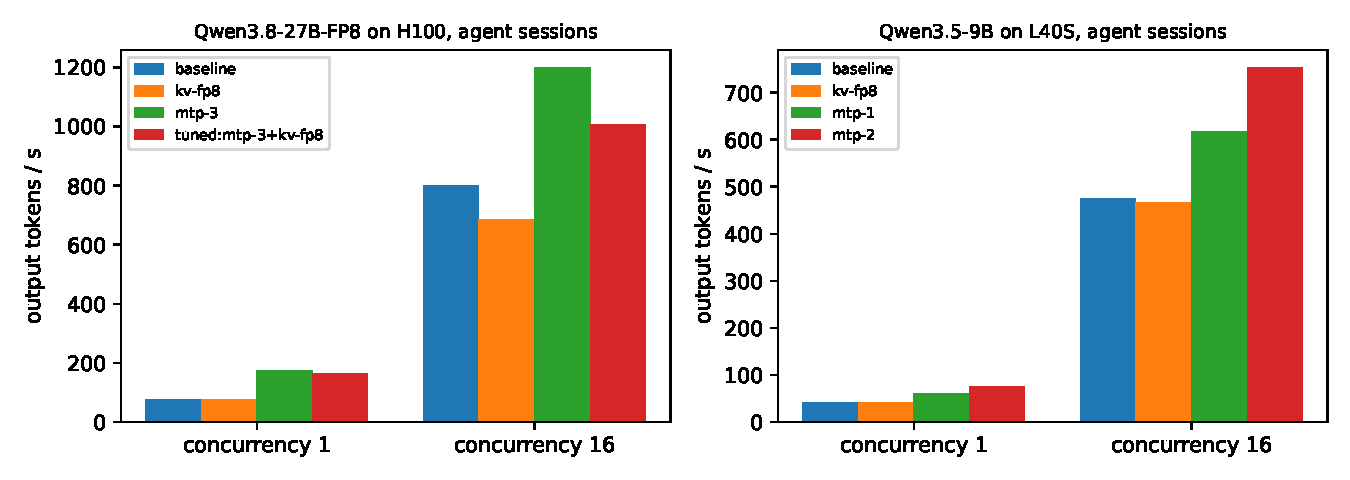
\includegraphics[width=\linewidth]{generated/fig_throughput.pdf}
\caption{Output tokens/s on the agent-session workload by profile. Single run per bar; no error bars yet.}\label{fig:throughput}
\end{figure}

\paragraph{Tail latency.} Tables~\ref{tab:ttft27} and~\ref{tab:ttft9} give p99 time to first token in seconds. A throughput gain can come with a larger tail, so both must be read together.

\begin{table}[h]\centering\small
\caption{Qwen3.8-27B-FP8: p99 time to first token (s).}\label{tab:ttft27}
\begin{tabular}{lrrrr}
\toprule
Profile & shared\_prefix, c=1 & shared\_prefix, c=16 & agent\_sessions, c=1 & agent\_sessions, c=16 \\
\midrule
baseline & 0.35 & 0.53 & 0.27 & 1.09 \\
kv-fp8 & 0.36 & 1.47 & 0.27 & 1.46 \\
mtp-3 & 0.36 & 0.79 & 0.28 & 0.94 \\
tuned:mtp-3+kv-fp8 & 0.37 & 1.51 & 0.29 & 1.20 \\
\bottomrule
\end{tabular}

\end{table}

\begin{table}[h]\centering\small
\caption{Qwen3.5-9B: p99 time to first token (s).}\label{tab:ttft9}
\begin{tabular}{lrrrr}
\toprule
Profile & shared\_prefix, c=1 & shared\_prefix, c=16 & agent\_sessions, c=1 & agent\_sessions, c=16 \\
\midrule
baseline & 0.53 & 0.69 & 0.41 & 0.95 \\
kv-fp8 & 0.58 & 1.39 & 0.43 & 1.42 \\
mtp-1 & 0.54 & 1.54 & 0.46 & 0.95 \\
mtp-2 & 0.57 & 0.84 & 0.45 & 0.74 \\
\bottomrule
\end{tabular}

\end{table}

\paragraph{Reading the numbers.} The same baseline profile, booted separately, reproduced within about 2\% in throughput, so we treat differences below roughly 5\% as noise and make no claim about them. The speculation gains (tens of percent to more than double) are far larger than this. We did not compute confidence intervals; the cells are single runs.

\subsection{A startup failure on a hybrid-attention model}\label{sec:startup}
With vLLM~0.33.0 defaults on one H100, the 27B model did not start. The engine stopped during CUDA-graph capture with
\begin{quote}\small\texttt{ValueError: max\_num\_seqs (1024) exceeds available Mamba cache blocks (745). Each decode sequence requires one Mamba cache block, so CUDA graph capture cannot proceed. Please lower max\_num\_seqs to at most 745 or increase gpu\_memory\_utilization.}\end{quote}
The default sequence limit (1024) exceeded the 745 recurrent-state blocks that fit alongside the weights and key-value cache. Setting \texttt{--max-num-seqs 512} resolved it, and it is part of our baseline.
We did not check whether this is documented upstream, nor how the threshold moves with GPU memory utilisation or context length.
A separate startup failure came from our own container image lacking a CUDA toolchain (\texttt{nvcc}); we mention it only because the symptom, an engine-initialisation error, is generic.

\subsection{Answer quality}\label{sec:quality}
Speculative decoding with verification is meant to preserve the output distribution, but an implementation can still differ, so we checked. We deployed the vanilla and the tuned (MTP) profile of each model behind an authenticated endpoint and asked the same 200 GSM8K test questions (fixed seed) at temperature 0 with thinking disabled, scoring exact match on the final number. Accuracy was 0.940 (vanilla) and 0.935 (MTP-3) for the 27B, and 0.900 and 0.910 for the 9B. The differences are one and two questions out of 200, within sampling noise, so we find no sign that speculation changed answer quality on this sample. We did not run this check for the FP8 key-value cache, which we do not recommend (it lowered throughput).

\section{Limitations}\label{sec:limits}
\begin{itemize}
  \item \textbf{Single short runs.} Each cell is one run of 24 requests (96 for 16 concurrent sessions). Baselines reproduced within about 2\% across boots, but run-to-run noise of the other profiles is not measured, so small differences are not evidence.
  \item \textbf{Two models, two GPUs, one engine version.} Results are for vLLM~0.33.0 and may not transfer to other engines (we did not run SGLang), models or hardware.
  \item \textbf{Synthetic prompts.} Random-word prompts control caching but have unnatural acceptance rates for speculative decoding. Replicating on real agent traces is future work.
  \item \textbf{p99 on small samples.} With 24 requests the nearest-rank p99 is the maximum.
  \item \textbf{Quality check is narrow.} One 200-question arithmetic sample at temperature 0 with thinking disabled; it does not cover long agent trajectories.
  \item \textbf{No end-to-end agent result.} We also ran a small pilot of a prompt-level agent harness on Terminal-Bench~2.1 and $\tau$-bench with the tuned engine. At the sample sizes we could afford (tens of tasks, one attempt each) it showed no statistically reliable difference, so it is not reported as a result and nothing here claims an agent-accuracy gain.
  \item \textbf{No production claim.} We did not measure long-running stability, failure rates or cost under real traffic.
\end{itemize}

\section{Reproducibility}
All code (profiles, workloads, sweep runner, analysis and this paper's table generator) and raw per-run results are in the repository
\todo{public repository URL and commit hash}. Tables and headline numbers in this paper are generated from the result files by \texttt{paper/make\_results.py}.

\bibliographystyle{plain}
\bibliography{refs}

\appendix
\section{Profiles}\label{app:profiles}
All profiles start from the baseline (Section~\ref{sec:setup}) and change only the listed flags; the full definitions are in \texttt{infer/profiles.py}.
\begin{center}\small\begin{tabular}{ll}\toprule
Profile & Change from baseline \\ \midrule
gpu-util-95 & \texttt{--gpu-memory-utilization 0.95} \\
kv-fp8 & \texttt{--kv-cache-dtype fp8} \\
seqs-256 / seqs-512 & \texttt{--max-num-seqs 256 / 512} \\
batched-8k / 16k & \texttt{--max-num-batched-tokens 8192 / 16384} \\
async-scheduling & \texttt{--async-scheduling} \\
no-prefix-cache & \texttt{--no-enable-prefix-caching} \\
mtp-$k$ & \texttt{--speculative-config} MTP with $k$ draft tokens \\
 & (method \texttt{mtp} on the 27B, \texttt{qwen3\_next\_mtp} on the 9B) \\
tuned (reported) & mtp-3 on the 27B, mtp-2 on the 9B \\ \bottomrule
\end{tabular}\end{center}

\end{document}
